\documentclass[12pt,letterpaper]{article}
\usepackage[T1]{fontenc}
\usepackage{microtype,amsmath,amssymb,amsthm,mathtools}
\usepackage{newtxtext,newtxmath}
\usepackage[letterpaper,margin=1in]{geometry}
\usepackage[hidelinks]{hyperref}
\usepackage{enumitem,booktabs,array}
\usepackage{tikz}
\newtheorem{theorem}{Theorem}[section]
\newtheorem{lemma}[theorem]{Lemma}
\newtheorem{proposition}[theorem]{Proposition}
\newtheorem{corollary}[theorem]{Corollary}
\theoremstyle{remark}
\newtheorem{remark}[theorem]{Remark}
\newcommand{\C}{\mathbb C}
\newcommand{\Hp}{H^\infty}
\newcommand{\D}{\mathcal D}
\DeclareMathOperator{\Dom}{Dom}
\DeclareMathOperator{\Ker}{Ker}
\DeclareMathOperator{\sgn}{sgn}
\title{Operator-Equivalence Classes of Grosswald--Schnitzer Prime Perturbations\\[0.45em]
\large Draft 2: Corrected and expanded version\\[0.25em]
\normalsize Weighted-transition criteria and a hierarchy of Sobolev-space comparisons}
\author{David Joyner\\\texttt{wdjoyner@gmail.com}}
\date{November 28, 2026 (expanded revision)}
\begin{document}
\maketitle
\begin{abstract}
This paper was expanded with assistance from ChatGPT (OpenAI); the specific contributions are described in the acknowledgments and revision log. 
For Grosswald--Schnitzer prime sequences $p_n\le a_n\le p_{n+1}$, we first define the generalized integers, the associated zeta function, and the generalized-prime summation operators, distinguishing literal convergent series from analytically continued symbol operators. In the companion Hardy-space realization, the analytic-symbol dilation operators are asserted to have the same closed joint zero-eigenspace. This conclusion depends on the closure and domain arguments of that working model, which are not independently reverified here. We distinguish this universal spectral equivalence from bounded \emph{diagonal left equivalence} of the full operator pairs. The latter is characterized by the quotient $Q_A/Q_B$ and its inverse being bounded on a right half-plane. We prove a quantitative necessary-and-sufficient summability criterion when the surviving Euler-factor logarithms are rationally independent. As a particularly concrete application, for perturbations replacing selected primes by the next prime, bounded comparability is equivalent to weighted summability of the discrete derivative of the difference of the two binary selection sequences. Hence moving \emph{every} prime to the next prime gives a bounded comparison, whereas moving alternating primes does not. We establish strict dependence of the resulting equivalence classes on the Sobolev index and discuss generic interior perturbations. The arguments are self-contained except for the previously established Hardy-space model and standard arithmetic facts. Originality and the relation to the Dirichlet-series/Bohr-lift literature require independent review; none of these results implies the Riemann hypothesis.
\end{abstract}

\setcounter{tocdepth}{2}
\tableofcontents

\section{Introduction}\label{sec:introduction}
\subsection{Motivation and principal results}
Zero-preservation of prime-perturbation zeta functions does not
automatically entail bounded equivalence of their summation operators.
This paper classifies bounded comparison for important perturbation families
using weighted transition sums and Euler-factor cancellation.
\subsection{Literature review}
Grosswald and Schnitzer established the original prime-gap
zero-preservation result \cite{GS78}.  Beurling's invariant-subspace
theory supplies useful operator-theoretic background \cite{Be49}.
The Bohr--Dirichlet-series literature concerns the independent
frequencies used below \cite{DGMS19,Sc20}.
The companion invariance note addresses the weaker zero-associated
spectral problem \cite{CJ26}. It relies on an unbounded-multiplier
realization, so its graph-core assumptions cannot be replaced
by equality of arithmetic zero sets.

The analytic theory of general Dirichlet series is treated in
\cite{DGMS19,Sc20}. The frequency-independence test below is
a specialized Euler-product question arising from that theory.
The formal RH development reported in \cite{LF26,Ru26}
affects the interpretation of the common zero exponents,
as explained in Section~\ref{sec:rh-2026}.

\paragraph{The November 2026 RH formalization.}
Alp\"oge's Claude-assisted Lean development was announced on
November 20, 2026. The Lean FRO and Mathlib Initiative certified
its RH statement and formal proof on November 21 \cite{LF26}.
Rubinstein reports independent machine checks of the original
and shortened formalizations \cite{Ru26}. The critical-line location
of nontrivial ordinary zeta zeros is therefore supported by certified
formal proof, although a complete human-readable exposition is still
being developed. The present paper does not audit the Lean development.
RH determines the location of the common zeta zeros. It does
\emph{not} imply boundedness of the Euler quotients, zero simplicity,
spectral synthesis, or similarity of the complete operator pairs.
\subsection{Background and a running example}
A prime-gap perturbation replaces the ordinary prime generator
\(p_n\) by a real number \(a_n\) between \(p_n\) and \(p_{n+1}\).
The resulting generalized integers are finite formal products.
The zeta function is their generating series, counting
multiplicities when different formal products coincide.

The principal example of cancellation is the endpoint sequence
\(a_n=p_{n+1}\), which moves every prime to its successor.
The quotient then telescopes:
\begin{equation}\label{eq:intro-telescope}
  Q_A(s)=\prod_{n\ge1}
  \frac{1-p_n^{-s}}{1-p_{n+1}^{-s}}
  =1-2^{-s}.
\end{equation}
The product is absolutely convergent for \(\Re s>1\).
The final expression continues it to \(\Re s>0\).
Infinitely many shifted generators therefore leave only one
noncanceled Euler factor.

\subsection{Notation and conventions}
The primes are $p_1=2<p_2=3<\cdots$.
A perturbation is $A=(a_n)$ with $p_n\le a_n\le p_{n+1}$.
Write $Q_A=\zeta_A/\zeta$ and $\delta=1/(2k)$.
For endpoint shifts $e_n\in\{0,1\}$,
$(\partial e)_j=e_j-e_{j-1}$ is their directed incidence boundary.
The space $H^\infty$ consists of bounded analytic functions
on the stated right half-plane.

\begin{center}
\begin{tabular}{@{}p{0.25\linewidth}p{0.65\linewidth}@{}}
\toprule
Symbol & Meaning\\
\midrule
\(A=(a_n)\), \(\mathcal N_A\) & Perturbed primes and
the multiset of generalized integers.\\
\(\zeta_A\), \(Q_A\) & Generalized zeta function
and the quotient \(Q_A=\zeta_A/\zeta\).\\
\(R_{A/B}\) & Comparison quotient \(Q_A/Q_B\)
for two perturbations.\\
\(S_k\), \(\delta\) & Weighted Sobolev space and
threshold \(\delta=1/(2k)\).\\
\(D_a\), \(T_A^{(r)}\) & Dilation by \(a\)
and the associated summation operator.\\
\(e\), \(\partial e\) & Endpoint shift pattern
and its signed incidence boundary.\\
\bottomrule
\end{tabular}
\end{center}
The distinction between a literal sum and an
analytically continued symbol is made in
Section~\ref{sec:definitions}.

\section[Prime perturbations and summation operators]{Definitions and examples: the perturbed primes and their summation operators}
\label{sec:definitions}

\subsection[The perturbed sequence]{What is $A$?}
Let $p_1=2,p_2=3,p_3=5,p_4=7,\ldots$ denote the usual primes.
A \emph{Grosswald--Schnitzer prime perturbation} is an indexed sequence
\begin{equation}\label{eq:Aprimes}
 A=(a_1,a_2,a_3,\ldots),\qquad p_n\le a_n\le p_{n+1}\quad(n\ge1).
\end{equation}
The numbers $a_n$ need not themselves be ordinary primes or even integers.
For instance, one may begin with $a_1=5/2$, $a_2=7/2$, and
$a_3=11/2$, then choose the remaining $a_n$ within their corresponding
prime gaps.  The notation $A$ always refers to the \emph{indexed
sequence}, not merely to a set of distinct real numbers: repetitions
can occur at a shared endpoint, such as $a_1=a_2=3$.

The \emph{generalized positive integers} generated by $A$ are the
finite products
\begin{equation}\label{eq:generalizedintegers}
 m=\prod_{j=1}^J a_j^{\nu_j},\qquad J\ge0,\quad \nu_j\in\mathbb Z_{\ge0}.
\end{equation}
Write $\mathcal N_A$ for this multiplicative \emph{multiset}; the empty
product is $1$, and different exponent vectors giving the same value
are counted with multiplicity.  For example, if $a_1=a_2=3$, then
$3$ occurs twice in $\mathcal N_A$ (once using each indexed generator).
If $A$ is the ordinary prime sequence, then $\mathcal N_A=\mathbb N$
with each positive integer occurring once.

For $\Re s>1$, the associated generalized zeta function is
\begin{equation}\label{eq:generalizedzeta}
 \zeta_A(s)=\sum_{m\in\mathcal N_A}m^{-s}
 =\prod_{n\ge1}(1-a_n^{-s})^{-1}.
\end{equation}
The sum uses multiplicities.  The Grosswald--Schnitzer theorem is
conveniently expressed through
\begin{equation}\label{eq:Qdefagain}
 Q_A(s)=\frac{\zeta_A(s)}{\zeta(s)}
 =\prod_{n\ge1}\frac{1-p_n^{-s}}{1-a_n^{-s}},\qquad \Re s>1;
\end{equation}
$Q_A$ admits a holomorphic, zero-free continuation to $\Re s>0$.
Consequently $\zeta_A$ and $\zeta$ have the same zeros, with
multiplicities, in that half-plane.

\subsection{The literal generalized-prime summation operator}
Fix $r\in\{2,3\}$.  Whenever the following series converge absolutely,
set
\begin{equation}\label{eq:literalTA}
 \boxed{\displaystyle
 (T_A^{(r)}f)(y)=\sum_{m\in\mathcal N_A}
 \left[f\!\left(\frac{y}{m}\right)
       -r f\!\left(\frac{y}{rm}\right)\right],\quad 0<y\le1.}
\end{equation}
The factor $r$ is the fixed integer used in the summation operator;
it is not a member of the perturbed-prime sequence by definition.
For $f(y)=y^s$ with $\Re s>1$, absolute convergence and
\eqref{eq:generalizedzeta} give
\begin{align}
 T_A^{(r)}y^s
 &=y^s\sum_{m\in\mathcal N_A}m^{-s}(1-r^{1-s})\notag\\
 &=\underbrace{(1-r^{1-s})\zeta_A(s)}_{m_{A,r}(s)}\,y^s.
 \label{eq:TApower}
\end{align}
Hence powers are eigenfunctions and the eigenvalue symbol is
\begin{equation}\label{eq:TAeigen}
 \boxed{m_{A,r}(s)=(1-r^{1-s})\zeta_A(s).}
\end{equation}
The use of $r=2$ and $r=3$ is especially useful: the two
auxiliary factors $1-2^{1-s}$ and $1-3^{1-s}$ have only the
common zero $s=1$, where the simple pole of $\zeta_A$
cancels it.  Thus the two \emph{analytic symbols} have no common
zeros except those of $\zeta_A$.

\subsection{Examples}
\paragraph{Example 1: the ordinary primes.}
For $A=(2,3,5,7,\ldots)$ we have $\mathcal N_A=\mathbb N$, and
\begin{align}
 T_A^{(r)}f(y)
 &=\sum_{n\ge1}f(y/n)-r\sum_{n\ge1}f(y/(rn))\notag\\
 &=\sum_{n\ge1}(1-r\,\mathbf1_{r\mid n})f(y/n).
 \label{eq:ordinarycase}
\end{align}
In particular, for $r=2$ the coefficients are $1,-1,1,-1,\ldots$:
\[
 T_A^{(2)}f(y)=f(y)-f(y/2)+f(y/3)-f(y/4)+\cdots,
\]
where the displayed rearrangement is justified when the relevant
series are absolutely convergent.

\paragraph{Example 2: all primes moved to their successors.}
If $a_n=p_{n+1}$ for every $n$, then
$A=(3,5,7,11,13,\ldots)$ and $\mathcal N_A$ consists precisely of
the positive \emph{odd} integers.  In this case
\[
 \zeta_A(s)=(1-2^{-s})\zeta(s),\qquad Q_A(s)=1-2^{-s},
\]
and
\begin{equation}\label{eq:oddTA}
 T_A^{(2)}f(y)=\sum_{\substack{m\ge1\\m\text{ odd}}}
 \left[f(y/m)-2f(y/(2m))\right].
\end{equation}
The symbol is
\[
 m_{A,2}(s)=(1-2^{1-s})(1-2^{-s})\zeta(s).
\]
This is also the simplest example of telescoping Euler-factor
cancellation, used below in the endpoint-equivalence classification.

\paragraph{Example 3: moving only the first prime.}
For $A=(5/2,3,5,7,11,\ldots)$, the generalized integers begin with
$1,5/2,3,5,25/4,15/2,\ldots$ (with their multiplicities).  We have
\begin{equation}\label{eq:oneprime}
 Q_A(s)=\frac{1-2^{-s}}{1-(5/2)^{-s}},\qquad
 m_{A,r}(s)=Q_A(s)(1-r^{1-s})\zeta(s).
\end{equation}
For instance $Q_A(2)=25/28$, so the nonzero eigenvalue on $y^2$
is multiplied by $25/28$ relative to the unperturbed operator.
Preserving the zero-associated eigenfunctions does \emph{not} mean
preserving all their nonzero eigenvalues.

\subsection{Analytic continuation: a necessary domain distinction}
The series \eqref{eq:literalTA} is defined directly only where its
convergence is justified.  In particular, \eqref{eq:TApower} follows
from ordinary absolute convergence for $\Re s>1$; one cannot simply
substitute a zeta zero $\rho$ with $0<\Re\rho<1$ into that infinite
series.  Instead, in the Sobolev-space operator theory developed below,
we use \emph{analytic-symbol operators}: define their action on the
algebraic domain
\[
 \mathcal D_k=\operatorname{span}\{y^s(\log y)^j:\Re s>1/(2k),\ j\ge0\}
\]
by
\begin{equation}\label{eq:TAderivative}
 \boxed{\displaystyle
 T_A^{(r)}\big(y^s(\log y)^j\big)
 =\frac{\partial^j}{\partial s^j}
       \big(m_{A,r}(s)y^s\big),\qquad \Re s>\frac1{2k}.}
\end{equation}
Here the symbol $m_{A,r}(s)=(1-r^{1-s})\zeta_A(s)$ is understood by
analytic continuation; its apparent singularity at $s=1$ is removable,
because $1-r^{1-s}$ cancels the simple pole of $\zeta_A$ there.
Formula \eqref{eq:TAderivative} agrees with the convergent summation
formula on powers and logarithmic powers when $\Re s>1$.
It does \emph{not}, by itself, prove that \eqref{eq:literalTA}
converges on all of $\mathcal D_k$ or defines the same closed operator
on larger function classes.  Establishing a natural regularized
summation realization is a separate research problem.

\section{Three different notions of equivalence}
Let $p_1=2<p_2=3<\cdots$ be the primes, and let $A=(a_n)$ be an admissible Grosswald--Schnitzer sequence,
\begin{equation}\label{eq:admissible}
 p_n\le a_n\le p_{n+1}.
\end{equation}
For $\Re s>1$ put
\begin{equation}\label{eq:Q}
 \zeta_A(s)=\prod_{n\ge1}(1-a_n^{-s})^{-1},\qquad
 Q_A(s)=\frac{\zeta_A(s)}{\zeta(s)}
 =\prod_{n\ge1}\frac{1-p_n^{-s}}{1-a_n^{-s}}.
\end{equation}
Grosswald--Schnitzer \cite{GS78} gives a holomorphic, nowhere-vanishing extension of $Q_A$ to $\Re s>0$. Let $\delta=1/(2k)$ for an integer $k\ge1$, and let $S_k$ be the full weighted Sobolev space of the companion notes,
\[
 \|f\|_{S_k}^2=\sum_{j=0}^k\int_0^1|f^{(j)}(y)|^2y^{2j-1-1/k}\,dy.
\]
On the exponential-polynomial domain $\D_k=\operatorname{span}\{y^s(\log y)^j:\Re s>\delta,\ j\ge0\}$, the operators have analytic symbols
\begin{equation}\label{eq:symbol}
 m_{A,r}(s)=Q_A(s)(1-r^{1-s})\zeta(s),\qquad r=2,3.
\end{equation}
We rely on the Hardy-space realization described in \cite{CJ26}: the closures $\overline{T_A^{(r)}}$ are boundedly conjugate (by an isomorphism independent of $A$) to adjoints of maximal Hardy multipliers. The joint closed kernels are independent of $A$.

We must \emph{not} confuse these three relations:
\begin{enumerate}[leftmargin=2em]
\item \textbf{Zero-model equivalence:} the closed joint kernels coincide for all $A$ (and hence have identical inherited norms). This is universal.
\item \textbf{Bounded diagonal left equivalence:} for $A,B$ a comparison operator $C_{A/B}$ acts on powers by
\[
 C_{A/B}y^s=R_{A/B}(s)y^s,\qquad R_{A/B}(s):=Q_A(s)/Q_B(s),
\]
 and extends boundedly and invertibly on $S_k$. We write $A\sim_\delta B$.
\item \textbf{Similarity of the full pairs:} the existence of a bounded invertible $S$ with $ST_B^{(r)}S^{-1}=T_A^{(r)}$. Left equivalence does \emph{not} assert this; in particular a comparison commuting with the dilation generator cannot produce a nontrivial similarity by conjugation.
\end{enumerate}
The earlier Hardy multiplier criterion yields the precise test
\begin{equation}\label{eq:Hinf}
 \boxed{A\sim_\delta B\quad\Longleftrightarrow\quad
 R_{A/B},\ R_{A/B}^{-1}\in H^\infty(\Re s>\delta).}
\end{equation}
It is immediately an equivalence relation. In terms of the analytic logarithm $\log R_{A/B}$, it is equivalent to uniform boundedness of $|\Re\log R_{A/B}(s)|$ for $\Re s>\delta$. The question is whether this analytic criterion admits an arithmetic description.

\section{A frequency-independent Euler-product theorem}
The following result supplies a sharp description for a broad and explicit family. It can be viewed as a consequence of Bohr's vertical-frequency principle \cite{DGMS19,Sc20}; for transparency, we prove it with bounded-harmonic means.

\begin{theorem}[Independent-frequency comparison criterion]\label{thm:independent}
Let $x_j\ge2$ be a countable family with $\{\log x_j\}$ linearly independent over $\mathbb Q$, and let $c_j\in\mathbb Z$ with
\[
 \sum_j|c_j|x_j^{-\sigma}<\infty\quad\hbox{for each }\sigma>1.
\]
Suppose the Euler product
\begin{equation}\label{eq:EulerF}
 F(s)=\prod_j(1-x_j^{-s})^{c_j},\qquad\Re s>1,
\end{equation}
continues holomorphically and without zeros to $\Re s>\delta$, where $0<\delta\le1$. Then
\begin{equation}\label{eq:maincriterion}
 \boxed{F,F^{-1}\in H^\infty(\Re s>\delta)
 \quad\Longleftrightarrow\quad\sum_j|c_j|x_j^{-\delta}<\infty.}
\end{equation}
Whenever these conditions hold, there are also exact supremum formulas:
\begin{align}
 \|F\|_{H^\infty(\Re>\delta)}
 &=\prod_{c_j>0}(1+x_j^{-\delta})^{c_j}
 \prod_{c_j<0}(1-x_j^{-\delta})^{c_j},\label{eq:norm1}\\
 \|F^{-1}\|_{H^\infty(\Re>\delta)}
 &=\prod_{c_j<0}(1+x_j^{-\delta})^{-c_j}
 \prod_{c_j>0}(1-x_j^{-\delta})^{-c_j}.\label{eq:norm2}
\end{align}
\end{theorem}
\begin{proof}
The weighted summability on the right of \eqref{eq:maincriterion} implies locally uniform absolute convergence of the logarithmic Euler product, uniformly on $\Re s\ge\delta$. The estimates $|\log(1-x^{-s})|\le (1-2^{-\delta})^{-1}x^{-\delta}$ show that both $F$ and its inverse are bounded.

For necessity, suppose both are bounded. Then $u(\sigma,t)=\log|F(\sigma+it)|$ is a \emph{bounded real-valued harmonic function} on $\sigma>\delta$, with $|u|\le M$. Fix a positive, translation-invariant mean $\mathcal M$ on bounded uniformly continuous functions of $t$ which agrees with the ordinary Ces\`aro mean for almost-periodic functions. One may obtain it by a weak-* cluster point of the averages over $[-T,T]$. For $\lambda\in\mathbb R$, put
\[
 a_\lambda(\sigma)=\mathcal M\big(u(\sigma,t)e^{-i\lambda t}\big).
\]
Interior derivative estimates for bounded harmonic functions justify differentiating with respect to $\sigma$ and integrating by parts under $\mathcal M$. Harmonicity gives
\[
 a_\lambda''(\sigma)=\lambda^2 a_\lambda(\sigma).
\]
Because $a_\lambda$ stays bounded for all $\sigma>\delta$, it contains no exponentially increasing solution. In the region $\sigma>1$, the absolutely convergent expansion
\[
 u(\sigma,t)=-\sum_j c_j\sum_{m\ge1}\frac{x_j^{-m\sigma}}{m}
 \cos(mt\log x_j)
\]
shows that $a_0(\sigma)=0$ and, for $\lambda=\pm m\log x_j$, the coefficient equals $-c_jx_j^{-m\sigma}/(2m)$. All other coefficients vanish. By the differential equation the same formulas hold on the entire region $\sigma>\delta$.

For a finite set $J$ of indices with nonzero $c_j$, define the nonnegative trigonometric polynomial
\[
 P_J(t)=\prod_{j\in J}\left(1-\sgn(c_j)\cos(t\log x_j)\right).
\]
Rational independence implies $\mathcal M(P_J)=1$. It also ensures that all Fourier frequencies involving two or more \emph{different} $\log x_j$ are distinct from $m\log x_\ell$, $m\ge1$. Hence the preceding Fourier-coefficient computation yields the exact identity
\[
 \mathcal M\big(u(\sigma,\cdot)P_J\big)
 =\frac12\sum_{j\in J}|c_j|x_j^{-\sigma}.
\]
Positivity of the mean and $|u|\le M$ now give
\[
 \sum_{j\in J}|c_j|x_j^{-\sigma}\le2M
 \qquad(\sigma>\delta).
\]
Let $J$ increase and $\sigma\downarrow\delta$. Monotone convergence proves necessity.

For \eqref{eq:norm1}--\eqref{eq:norm2}, each factor has maximum modulus $1+x_j^{-\sigma}$ or reciprocal maximum $(1-x_j^{-\sigma})^{-1}$ according to the sign of $c_j$. Rational independence and Kronecker's theorem let the phases of any finite family approach these optimal values simultaneously. Uniform convergence of the logarithmic product under the summability condition controls the tail. Maximizing over $\sigma>\delta$ then gives the asserted products.
\end{proof}

\begin{remark}[Why both bounds matter]
The necessity proof uses $\log|F|$ bounded \emph{above and below}. A one-sided $H^\infty$ hypothesis alone does not lead to the same two-sided summability criterion. The theorem is about boundedly invertible comparison multipliers, not merely bounded ones.
\end{remark}

\paragraph{Worked example (two independent frequencies).}
Take
\[
 F(s)=\frac{1-2^{-s}}{1-3^{-s}}.
\]
The logarithms of \(2\) and \(3\) are rationally independent,
and the signed inventory consists of \(+1\) at \(2\) and
\(-1\) at \(3\). Hence \(F\) and \(F^{-1}\) are bounded
on every half-plane \(\Re s>\delta>0\).
For \(0<\delta\le1\), the exact norm formula yields
\[
 \|F\|_{H^\infty(\Re s>\delta)}
 =\frac{1+2^{-\delta}}{1-3^{-\delta}}.
\]
This simple comparison illustrates the sign convention
in Theorem~\ref{thm:independent}.

\section{Exact classification for endpoint perturbations}\label{sec:endpoint}
Fix a binary sequence $e=(e_n)_{n\ge1}\in\{0,1\}^{\mathbb N}$, and set
\begin{equation}\label{eq:endpoint}
 a_n(e)=p_{n+e_n}.
\end{equation}
Thus $e_n=1$ means ``move $p_n$ to the next prime,'' while $e_n=0$ means ``leave $p_n$ unchanged.'' Put $e_0=0$ and define the discrete derivative
\[
 d_j(e)=e_j-e_{j-1}\in\{-1,0,1\},\qquad j\ge1.
\]
On $\Re s>1$, regrouping the absolutely convergent factors gives
\begin{equation}\label{eq:endpointfactor}
 Q_e(s)=\prod_{j\ge1}(1-p_j^{-s})^{d_j(e)}.
\end{equation}
This factorization reveals exact cancellation between neighboring shifts.

\begin{theorem}[Weighted-transition classification]\label{thm:transition}
For binary endpoint perturbations $e,f$, and any $\delta>0$, the following are equivalent:
\begin{enumerate}[label=(\roman*),leftmargin=2em]
\item The diagonal comparison $Q_e/Q_f$ is bounded and boundedly invertible on $\Re s>\delta$.
\item The full analytic-symbol operator pairs are boundedly diagonally left equivalent on the corresponding Hardy/Sobolev model (when $\delta=1/(2k)$).
\item The difference of the shift patterns has summable \emph{weighted variation}:
\begin{equation}\label{eq:BV}
 \boxed{\sum_{j\ge1}p_j^{-\delta}
 \left|(e_j-f_j)-(e_{j-1}-f_{j-1})\right|<\infty.}
\end{equation}
\end{enumerate}
The exact comparison-symbol norms are given by \eqref{eq:norm1}--\eqref{eq:norm2} with $x_j=p_j$ and $c_j=d_j(e)-d_j(f)$.
\end{theorem}
\begin{proof}
Use \eqref{eq:endpointfactor} to write $Q_e/Q_f$ as \eqref{eq:EulerF}, with $x_j=p_j$ and $c_j=d_j(e)-d_j(f)$. Unique factorization of integers makes $\{\log p_j\}$ rationally independent. Theorem~\ref{thm:independent} proves (i)$\Longleftrightarrow$(iii), while the Hardy comparison criterion \eqref{eq:Hinf} proves (i)$\Longleftrightarrow$(ii).
\end{proof}

\begin{corollary}[Individual classes relative to ordinary primes]\label{cor:blocks}
An endpoint perturbation $e$ is comparable with the unperturbed primes on $S_k$ precisely when
\[
 \sum_{j:\,e_j\ne e_{j-1}}p_j^{-1/(2k)}<\infty.
\]
Thus the appropriate invariant is the \emph{density of beginnings and ends of runs}, not the total number of primes moved.
\end{corollary}

\paragraph{Example A: all primes moved, yet equivalent.}
If $e_j=1$ for every $j$, all factors telescope:
\[
 Q_e(s)=1-2^{-s}.
\]
This and its reciprocal belong to $H^\infty(\Re s>\delta)$ for \emph{every} $\delta>0$. The perturbation changes infinitely many primes, but has only one surviving transition in the Euler-factor inventory.

\paragraph{Example B: alternating primes, inequivalent.}
Let $e_j=1$ for odd $j$ and $e_j=0$ for even $j$. Then $|d_j(e)|=1$ for every $j$. Since $\sum_p p^{-\delta}=\infty$ for $0<\delta\le1$, Theorem~\ref{thm:transition} implies $e\not\sim_\delta0$ for all the Sobolev values $\delta=1/(2k)$.

\paragraph{Example C: runs and telescoping.}
If the ones form finite consecutive runs $[a_\ell,b_\ell]$ separated by at least one zero, then
\[
 Q_e(s)=\prod_\ell\frac{1-p_{a_\ell}^{-s}}{1-p_{b_\ell+1}^{-s}}.
\]
The weighted-transition test becomes summability of the $p_{a_\ell}^{-\delta}$ and $p_{b_\ell+1}^{-\delta}$ terms. Long blocks may be harmless if their endpoints are sufficiently sparse.


\section[Graph flows and transfer operators]{Graph-theoretic interpretation: prime flows, boundaries, and transfer operators}\label{sec:graph}
\label{sec:prime-graphs}

The arithmetic equivalence classes admit a direct interpretation in terms of
flows and incidence operators on a countable directed graph.  This description
is useful in three ways: it explains Euler-factor cancellation, gives a
quantitative stability bound, and supplies finite graph models of the
literal summation operators.

\subsection{The prime path and its incidence boundary}

Let \(G_P\) be the directed ray with vertices \(v_j=p_j\) and edges
\(b_j:p_j\to p_{j+1}\), \(j\ge1\).  For an endpoint perturbation
\(a_j=p_{j+e_j}\), put the binary flow \(e_j\in\{0,1\}\) on \(b_j\).
We use the incidence convention
\[
 (\partial e)_j=e_j-e_{j-1},\qquad e_0=0,
\]
so an occupied edge contributes \(+1\) at its source and \(-1\) at its
target.  This is the (signed) vertex boundary of the edge flow.

\begin{center}
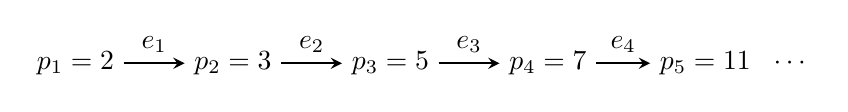
\begin{tikzpicture}[>=stealth,baseline]
\node (a) at (0,0) {$p_1=2$};
\node (b) at (2,0) {$p_2=3$};
\node (c) at (4,0) {$p_3=5$};
\node (d) at (6,0) {$p_4=7$};
\node (e) at (8,0) {$p_5=11$};
\draw[->,thick] (a)--node[above]{$e_1$}(b);
\draw[->,thick] (b)--node[above]{$e_2$}(c);
\draw[->,thick] (c)--node[above]{$e_3$}(d);
\draw[->,thick] (d)--node[above]{$e_4$}(e);
\node at (9.1,0) {$\cdots$};
\end{tikzpicture}
\end{center}

Put \(g_s(x)=\log(1-x^{-s})\), with the branch specified by its
convergent power series for \(x>1\) and \(\Re s>0\).
An elementary discrete-Stokes formula is
\begin{equation}\label{eq:graph-stokes}
 \sum_{n=1}^{N}e_n\bigl(g_s(p_n)-g_s(p_{n+1})\bigr)
 =\sum_{j=1}^{N}(\partial e)_j g_s(p_j)
       -e_Ng_s(p_{N+1}).
\end{equation}
The left side converges absolutely and locally uniformly for \(\Re s>0\).
Indeed, on a compact subset of that half-plane,
\[
 |g'_s(x)|\le C_K x^{-1-\sigma_K}\quad(x\ge2)
\]
for some \(\sigma_K>0\), and
\(\sum_n\int_{p_n}^{p_{n+1}}x^{-1-\sigma_K}\,dx<\infty\).
Since \(g_s(p_n)\to0\), taking \(N\to\infty\) in
\eqref{eq:graph-stokes} gives
\begin{equation}\label{eq:graph-product}
 \boxed{\quad
 \log Q_e(s)
 =\sum_{n\ge1}e_n\bigl[g_s(p_n)-g_s(p_{n+1})\bigr]
 =\sum_{j\ge1}(\partial e)_j g_s(p_j),\quad \Re s>0.
 \quad}
\end{equation}
The second series in \eqref{eq:graph-product} need not be absolutely
convergent: its equality follows from the boundary term in
\eqref{eq:graph-stokes}, not from arbitrary rearrangement.

For \(e_n=1\) on every edge, the interior boundary vanishes and
\(\partial e=(1,0,0,\ldots)\).  Therefore
\[
 \log Q_e(s)=g_s(2),\qquad Q_e(s)=1-2^{-s}.
\]
An infinite occupied ray has only a finite source boundary.  If instead
\(e_n=1\) precisely for \(u\le n\le v\), then
\[
 \partial e=\mathbf 1_{\{u\}}-\mathbf 1_{\{v+1\}},
 \qquad Q_e(s)=\frac{1-p_u^{-s}}{1-p_{v+1}^{-s}}.
\]
For alternating occupied edges, the graph boundary is supported at
every vertex, explaining why cancellation is much weaker.

\subsection{Weighted graph variation and quantitative conditioning}

For a bounded integer-valued edge flow \(h=(h_j)\), let
\begin{equation}\label{eq:graph-TV}
 V_\delta(h):=\sum_{j\ge1}p_j^{-\delta}
                  |h_j-h_{j-1}|,\qquad h_0=0,\quad\delta>0.
\end{equation}
This is the weighted \(\ell^1\)-norm of its incidence boundary,
a discrete bounded-variation quantity on \(G_P\).
For binary perturbations \(e,f\), the previously established endpoint
classification is exactly \(e\sim_\delta f\) if and only if
\(V_\delta(e-f)<\infty\).  In particular, its invariant is a
\emph{boundary norm}, not the number or size of occupied edges.

\begin{proposition}[Graph-variation stability bound]
\label{prop:graph-conditioning}
Let \(e,f\) be endpoint perturbations and \(0<\delta\le1\).
If \(V_\delta(e-f)<\infty\), then
\(R_{e/f}=Q_e/Q_f\) and its inverse belong to
\(H^\infty(\Re s>\delta)\), and
\begin{equation}\label{eq:graph-stability}
 \max\{\|R_{e/f}\|_\infty,\|R_{e/f}^{-1}\|_\infty\}
 \le \exp\!\left(\frac{V_\delta(e-f)}{1-2^{-\delta}}\right).
\end{equation}
The product of the two operator-multiplier norm bounds is at most
\(\exp(2V_\delta(e-f)/(1-2^{-\delta}))\).
\end{proposition}
\begin{proof}
Put \(h=e-f\), and \(c_j=h_j-h_{j-1}\).
For \(\Re s>\delta\), the estimate
\[
 |\log(1-p_j^{-s})|
 \le \frac{p_j^{-\delta}}{1-p_j^{-\delta}}
 \le \frac{p_j^{-\delta}}{1-2^{-\delta}}
\]
shows that \(\sum_j c_jg_s(p_j)\) converges absolutely and uniformly
and has modulus at most
\(V_\delta(h)/(1-2^{-\delta})\).
Exponentiate \eqref{eq:graph-product} for the quotient, and then
apply the same argument with \(-h\).
\end{proof}

The additive group of bounded integer edge flows contains the subgroup
\(\{h:V_\delta(h)<\infty\}\).
Consequently the binary endpoint perturbations map to equivalence
classes in the quotient by this subgroup.  This is a convenient
graph-cochain description of the arithmetic classification; it does
\emph{not} assert ordinary graph-Laplacian spectral equivalence.

\subsection{A signed-frequency graph for arbitrary interior shifts}

The same bookkeeping works beyond the endpoints.  For a finite
perturbation \(A_N=(a_1,\ldots,a_N)\), draw the oriented edge
\(p_n\to a_n\) on the vertex set of all distinct frequencies
\(\{p_1,\ldots,p_N,a_1,\ldots,a_N\}\).  A loop contributes zero.
The signed vertex boundary is the atomic measure
\[
 \mu_{A,N}:=\sum_{n=1}^N(\delta_{p_n}-\delta_{a_n}).
\]
For every \(\Re s>0\), the finite Euler quotient satisfies
\begin{equation}\label{eq:graph-atomic}
 \log Q_{A,N}(s)=
 \int_{(1,\infty)}\log(1-x^{-s})\,d\mu_{A,N}(x).
\end{equation}
If two edges share a frequency endpoint, their incidence
coefficients may cancel.  With rational independence of distinct
surviving logarithmic frequencies, the weighted signed-inventory
criterion from the companion equivalence-class argument is precisely
summability of this atomic boundary with weight \(x^{-\delta}\).
Without that independence, no general necessity assertion follows
from the graph model alone.

\subsection{The multiplicative graph of generalized integers}

For \(A_N=(a_1,\ldots,a_N)\), consider the graded directed graph
\[
 \Gamma_{A_N}:\quad
 V=\mathbb Z_{\ge0}^{N},\qquad
 \nu\longrightarrow \nu+\mathbf e_j\quad(1\le j\le N).
\]
Give the vertex \(\nu\) the weight
\(w_s(\nu)=\prod_{j=1}^N a_j^{-s\nu_j}\).
Summing \emph{vertices}, rather than all directed paths, gives
\begin{equation}\label{eq:graph-vertexzeta}
 \sum_{\nu\in\mathbb Z_{\ge0}^N}w_s(\nu)
 =\prod_{j=1}^N(1-a_j^{-s})^{-1}
 =\zeta_{A,N}(s),\qquad\Re s>0.
\end{equation}
This vertex interpretation respects the multiplicities of
generalized integers.  For example, \(a_1=a_2=3\) produces
three exponent vectors of total degree two, all evaluating to \(9\);
accordingly the coefficient of \(3^{-2s}\) in
\((1-3^{-s})^{-2}\) is \(3\).  Counting directed paths instead
would introduce different, and incorrect, multiplicities.
The graph in \eqref{eq:graph-vertexzeta} is not an Ihara
nonbacktracking-cycle zeta construction.

\begin{proposition}[Convergent graph-transfer realization]
\label{prop:graph-transfer}
For \(\sigma>1\), let \(X_\sigma\) be the Banach space of functions
on \((0,1]\) with
\[
 \|f\|_{X_\sigma}:=\sup_{0<y\le1}y^{-\sigma}|f(y)|<\infty.
\]
Write \(D_a f(y)=f(y/a)\).  The operator products
\begin{equation}\label{eq:graph-resolvents}
 P_A=\prod_{n\ge1}(I-D_{a_n})^{-1},
 \qquad
 (I-qD_q)P_A\quad(q=2,3)
\end{equation}
converge in operator norm on \(X_\sigma\), and
\begin{equation}\label{eq:graph-literalsum}
 (I-qD_q)P_Af(y)
 =\sum_{m\in\mathcal N_A}
 \left[f(y/m)-qf(y/(qm))\right].
\end{equation}
All sums in \eqref{eq:graph-literalsum} converge absolutely in
\(X_\sigma\).  These operators are boundedly invertible on
\(X_\sigma\).
\end{proposition}
\begin{proof}
The dilation operators commute and
\(\|D_a\|_{X_\sigma}=a^{-\sigma}\).
Since \(a_n\ge p_n\) and
\(\sum_n p_n^{-\sigma}<\infty\), the two products
\(\prod_n(I-D_{a_n})^{-1}\) and
\(\prod_n(I-D_{a_n})\) converge in operator norm and
are inverses.  Expand each geometric series and pass to the
norm limit to obtain the generalized-integer sum with
multiplicity.  Finally,
\(\|qD_q\|=q^{1-\sigma}<1\), so \(I-qD_q\) is invertible
by a Neumann series.
\end{proof}

\begin{remark}[Scope of the graph model]
The space \(X_\sigma\), \(\sigma>1\), is the domain of an
\emph{absolutely convergent} graph-transfer representation.  It
does not contain the zeta-zero eigenfunctions \(y^\rho\) from the
critical strip and is not a substitute for the analytically
continued \(S_k\) operators.  In particular, Proposition
\ref{prop:graph-transfer} proves no kernel invariance in the
critical strip.  It supplies a natural discrete approximation
and separates the convergent graph mechanics from the deeper
operator-domain problem.
\end{remark}

\paragraph{Further graph questions.}
One can ask whether (i) weighted incidence-boundary classes
admit computable finite-section approximations with certified
tails; (ii) equality of closed graph-transfer domains forces
bounded comparison in a natural completion; and (iii) the
graph boundary at infinity controls comparison-operator
conditioning.  These are proposed investigations, not claims
about the spectrum of a graph Laplacian.

\section{The Sobolev index yields a strict hierarchy}
Write $\delta_k=1/(2k)$. As $k$ grows, $\delta_k$ decreases and the weight $p^{-\delta_k}$ increases. Consequently
\[
 e\sim_{\delta_{k+1}}f\quad\Longrightarrow\quad e\sim_{\delta_k}f,
\]
but the reverse is generally false.

\begin{proposition}[A concrete strict separation]\label{prop:strict}
There exists an endpoint perturbation $e$ for which $e\sim_{1/2}0$ but $e\not\sim_{1/4}0$. Specifically, take the set of indices at which $e_n=1$ to be $\{\lceil j^3\rceil:j\ge2\}$, and take $e_n=0$ elsewhere, ignoring any finitely many initial collisions.
\end{proposition}
\begin{proof}
For large $j$ each isolated $1$ causes two transitions, at $n_j=\lceil j^3\rceil$ and $n_j+1$. The prime number theorem gives $p_{n_j}\asymp j^3\log j$ and $p_{n_j+1}\asymp j^3\log j$. Thus the weighted variation has the same convergence as
\[
 \sum_{j\ge2}j^{-3\delta}(\log j)^{-\delta}.
\]
This series converges for $\delta=1/2$, and diverges for $\delta=1/4$, proving the claim by Theorem~\ref{thm:transition}.
\end{proof}

More generally, the threshold $\inf\{\alpha>0:\sum_j|d_j(e)-d_j(f)|p_j^{-\alpha}<\infty\}$ is a numerical \emph{comparison exponent} for endpoint sequences; behavior at the threshold must be checked separately.

\section{Generic interior perturbations and a common arithmetic invariant}
Endpoint sequences are highly structured because adjacent prime factors may cancel. At the other extreme, choose each changed $a_n$ in the open interval $(p_n,p_{n+1})$ so that its logarithm, together with the prime logarithms and the logarithms of other chosen interior values, is rationally independent. This is possible even with $0<a_n-p_n<2^{-n}$, since at each stage only countably many forbidden choices arise. Such independence is also generic in the Baire-category sense and under independent absolutely continuous random choices.

For an arbitrary admissible sequence $A$, let
\[
 r_n(A)=\mathbf 1_{\{a_n>p_n\}},\quad
 e_n(A)=\mathbf1_{\{a_n=p_{n+1}\}},\quad e_0(A)=0,
\]
and let $I(A)=\{n:p_n<a_n<p_{n+1}\}$. By grouping endpoint contributions,
\begin{equation}\label{eq:inventory}
 Q_A(s)=\left(\prod_{j\ge1}(1-p_j^{-s})^{r_j(A)-e_{j-1}(A)}\right)
 \left(\prod_{n\in I(A)}(1-a_n^{-s})^{-1}\right),\qquad\Re s>1.
\end{equation}
For a pair $A,B$, cancel any identical interior factors in $Q_A/Q_B$. Let $c_x$ be the remaining signed exponent of $(1-x^{-s})$ at each ordinary prime $x=p_j$ and each distinct interior point $x$.

\begin{corollary}[Generic signed-Euler-inventory classification]\label{cor:inventory}
If the logarithms of all distinct interior points occurring in $A$ or $B$ are, jointly with the prime logarithms, rationally independent, then
\begin{equation}\label{eq:inventorycriterion}
 \boxed{A\sim_\delta B\quad\Longleftrightarrow\quad
 \sum_{x:\,c_x\ne0}|c_x|x^{-\delta}<\infty.}
\end{equation}
The formula includes the pure endpoint case as a special case.
\end{corollary}
\begin{proof}
After combining duplicate Euler factors, \eqref{eq:inventory} for $Q_A/Q_B$ takes the form \eqref{eq:EulerF}. There are only boundedly many factors per prime interval, so $\sum_x|c_x|x^{-\sigma}<\infty$ for $\sigma>1$. Apply Theorem~\ref{thm:independent} and \eqref{eq:Hinf}.
\end{proof}

\begin{corollary}[Generic dense interior shifts are never boundedly comparable]\label{cor:dense}
Suppose $a_n\in(p_n,p_{n+1})$ for every $n$, with the rational independence stipulated above. Then $Q_A,1/Q_A$ cannot both be bounded on $\Re s>\delta$ for any $0<\delta\le1$, even if $a_n-p_n\to0$ faster than any prescribed positive summable sequence.
\end{corollary}
\begin{proof}
Here the signed inventory contains the prime factors with coefficient $+1$ and the interior factors with coefficient $-1$. In particular, its weighted sum contains $\sum_p p^{-\delta}=\infty$ for $\delta\le1$. The corollary follows from \eqref{eq:inventorycriterion}.
\end{proof}

\section[Full-operator consequences]{Consequences for the full operators and unresolved classification questions}
For $A\sim_\delta B$, the boundedly invertible comparison $C_{A/B}$ maps $\D_k$ into itself and commutes with each analytic-symbol operator on this domain. Passing to closures yields the \emph{left-equivalence identities}
\begin{equation}\label{eq:lefteq}
 \overline{T_A^{(r)}}=C_{A/B}\overline{T_B^{(r)}},\qquad
 \Dom\overline{T_A^{(r)}}=\Dom\overline{T_B^{(r)}},\qquad r=2,3.
\end{equation}
Indeed $C_{A/B}$ is bounded and has a bounded inverse, so it preserves graph convergence in both directions. The associated graph norms are equivalent, and this applies to the joint graph domain as well. If $A\not\sim_\delta B$, this only proves that the \emph{canonical diagonal comparison} is not boundedly invertible. It does \emph{not} by itself prove different maximal operator domains, nor rule out a nondiagonal similarity.

The classification gives the following hierarchy:
\begin{center}
\begin{tabular}{@{}p{0.37\linewidth}p{0.49\linewidth}@{}}
\toprule
\textbf{Level} & \textbf{Behavior under prime perturbations}\\
\midrule
Joint closed zero-model & Identical in the companion model, subject to its closure and domain hypotheses\\
Bounded diagonal left equivalence & Nontrivial classes; exact weighted-variation criterion for endpoint shifts and weighted-inventory criterion for independent frequencies\\
Full-pair similarity, resolvents, pseudospectra & Not classified by these results\\
\bottomrule
\end{tabular}
\end{center}

\paragraph{Research directions.} The next steps are to (a) remove the independence hypothesis using relations among interior Euler frequencies; (b) test whether equality of \emph{full graph domains} forces bounded diagonal comparability, possibly for the pair of symbols rather than either one separately; (c) classify perturbations under a stronger requirement that resolvents or pseudospectra be quantitatively comparable; and (d) relate the signed Euler inventories to the Bohr transform and Dirichlet-series multiplier literature. These problems may lead to a more meaningful operator taxonomy than zero preservation alone.

\paragraph{Status and scope.} The weighted-transition theorem and its proof are offered as a concrete research development, not as a verified publication-novel theorem. The arithmetic independence assumptions are essential to the general inventory criterion, and assertions about similarity must not be inferred from left equivalence. The operators $T_A^{(r)}$ are defined through their analytic symbols; this does not assert convergence of a naive generalized-prime dilation series on the full common domain.


\section[The November 2026 RH development]{Consequences of the November 2026 RH formalization}
\label{sec:rh-2026}
On November 20, 2026 Levent Alp\"oge reported a formal proof of the
Riemann hypothesis (RH) developed with Claude.  The Lean FRO and
Mathlib Initiative certified the correctly stated and machine-checked
RH proof on November 21 \cite{LF26}.  Rubinstein independently reports
checks of the original and shortened formalizations \cite{Ru26}.
Human-readable proofs are still being developed.  The present paper
does not purport to independently check the large Lean development.

Taking the certified formal RH theorem \cite{LF26,Ru26} as
an external input,\footnote{This paper does not itself prove RH
or independently verify the Lean development. The November 2026
certification concerns RH, not the additional operator-theoretic
assertions studied here.} every nontrivial zeta zero is
$\rho=\frac12+i\gamma$.  For $k\ge2$ the Sobolev threshold
$\delta=1/(2k)$ is strictly below $\frac12$, and all zero-powers
are algebraically admissible.  For $k=1$ the threshold equals
$\frac12$, so none of these zero-powers satisfies the strict
domain inequality.  This sharpens the spectral-model discussion
but does not, by itself, prove spectral synthesis or a statement
about the closed joint kernel.

Grosswald--Schnitzer zero preservation then places the nontrivial
zeros of each $\zeta_A$ in $\Re s>0$ on the same critical line,
with the same multiplicities and ordinates as $\zeta$.
RH does not imply that these zeros are simple, so logarithmic
generalized eigenvectors cannot simply be discarded.
The shifted dilation generator $-i(\Delta-\frac12)$ has real
eigenvalues $\gamma$ on its admissible zero-power eigenvectors,
but need not be symmetric or self-adjoint.

RH neither makes the Euler quotient $Q_A$ or its reciprocal
bounded nor changes the graph-boundary summability test.
It does not establish boundedly invertible similarity of the
full summation operators, equality of their nonzero spectra,
equivalence of graph domains, or pseudospectral stability.
The ordinary-prime conditional bounds
$\psi(x)=x+O(x^{1/2}\log^2x)$ and
$\pi(x)=\operatorname{Li}(x)+O(x^{1/2}\log x)$
do not transfer to arbitrary Beurling or random prime systems
without additional comparison estimates.
The announced Dirichlet-$L$ GRH is a separate result and should
not be identified with a claim for all generalized zeta functions.

\section{Summary of results and open questions}\label{sec:summary}
The bounded diagonal comparison relation separates three
operator-theoretic notions. Equality of the zero-associated
closed kernel belongs to the companion Hardy-space model,
subject to its domain and closure results. Bounded diagonal
left equivalence is characterized by two-sided \(H^\infty\)
bounds for the quotient of Euler symbols.
Similarity of the complete operator pairs is not established.

For endpoint shifts, Theorem~\ref{thm:transition} gives an
exact weighted-transition test. The prime-path graph
explains cancellation within runs of shifted primes.
For independent interior frequencies,
Corollary~\ref{cor:inventory} gives a corresponding signed
Euler-factor inventory criterion. The strict hierarchy
in Proposition~\ref{prop:strict} shows that the classes
depend on Sobolev regularity.

Further work should characterize operator graph domains
without requiring a prescribed diagonal comparison.
Other open problems include interior shifts with rationally
dependent frequencies and stability of resolvents and
pseudospectra. Matching arithmetic zero sets does not
resolve any of these questions.

\section{Glossary of technical terms}
The following definitions supplement the main text for readers
whose background is in analysis rather than generalized-prime systems.
\begin{description}[style=nextline,leftmargin=1.5em]
\item[Analytic continuation] Extension of a function beyond its original convergence domain. The continued function need not be represented by the original infinite series.
\item[Blaschke product] An inner function built from a zero sequence satisfying the Blaschke condition. Its model space records the zero set with multiplicity.
\item[Bounded diagonal comparison] A comparison quotient and its reciprocal both belong to $H^\infty$ on the chosen half-plane. It gives invertible left equivalence, not generally operator similarity.
\item[Critical line] The line $\Re s=\tfrac{1}{2}$. RH puts the nontrivial ordinary zeta zeros there.
\item[Discrete divergence] The signed incidence boundary of an edge flow. The source and target contributions telescope along prime-path blocks.
\item[Euler-factor inventory] The signed frequencies remaining after cancellation of two Euler products. Its weighted size can control boundedness of a multiplier.
\item[Exponent-vector graph] The directed lattice of formal generalized integers. Its vertex generating series produces the Euler product with multiplicity.
\item[Graph norm] The norm \(\|f\|_T=(\|f\|^2+\|Tf\|^2)^{1/2}\) on the domain of an operator. It compares operator domains and can distinguish closed realizations even when their point spectra coincide.
\item[Hardy space] A Hilbert space of analytic functions with square-integrable boundary behavior. Its multiplication operators provide the model for dilation symbols.
\item[Inner factor] A factor with boundary modulus one almost everywhere. Its Blaschke and singular components determine invariant-subspace phenomena.
\item[Joint kernel] The intersection of several operator null spaces. Pairing $q=2$ and $q=3$ removes extraneous zeros of the auxiliary factors.
\item[Operator domain] The subspace on which an unbounded operator acts. A multiplier prescription on powers is not automatically a closed operator.
\item[Outer function] A Hardy or Smirnov function determined by its boundary modulus up to phase. Outerness does not mean bounded invertibility.
\item[Pseudospectrum] The region of large resolvent norms or spectral instability under small perturbations. It is not fixed by the zeros of arithmetic symbols.
\item[Riesz basis] The boundedly invertible image of an orthonormal basis. Having complete root vectors is weaker.
\item[Self-adjointness] Equality of an operator and its Hilbert-space adjoint, including domains. Real eigenvalues are not sufficient.
\item[Smirnov class] Ratios of bounded analytic functions with an outer denominator. This allows useful unbounded analytic quotients in the Hardy model.
\item[Sobolev threshold] The strict exponent condition $\Re s>1/(2k)$. When $k=1$ the RH critical line lies on its boundary.
\item[Spectral synthesis] Completeness of generalized eigenfunctions within the relevant invariant subspace. It requires more than matching zero sets.
\item[Weighted graph variation] A sum of weighted absolute incidence jumps. It quantifies Euler-factor cancellation for endpoint perturbations.
\item[Zero multiplicity] The vanishing order of an analytic function at a zero. Multiple zeros produce logarithmic generalized eigenvectors.
\item[Almost-periodic function] A function obtained as a uniform limit of finite trigonometric sums, in the sense of Bohr. A translation-invariant mean extracts its frequencies and is used in the comparison theorem.
\item[Beurling generalized primes] Abstract real generators greater than one from which a multiplicative system is built. Their finite formal products are generalized integers and are counted with multiplicity.
\item[Bohr transform] An identification of Dirichlet-frequency coefficients with monomials on a torus or polydisk. It motivates why rational independence permits independent finite-phase approximations.
\item[Dirichlet series] A series of the form \(\sum a_n e^{-\lambda_n s}\) with real frequencies \(\lambda_n\). For the ordinary integers one has \(\lambda_n=\log n\).
\item[Endpoint shift] A perturbation that leaves \(p_n\) fixed or replaces it with \(p_{n+1}\). The binary edge-flow representation makes consecutive shifts telescope.
\item[Generalized integer] A finite formal product of generalized primes, described by a nonnegative exponent vector. Two vectors can have the same numerical product, so the generating series counts both.
\item[Holomorphic symbol] An analytic function prescribing an operator's action on powers \(y^s\). This prescription need not agree with a pointwise-convergent summation series outside the original convergence half-plane.
\item[Kronecker approximation] A density theorem for rotations with rationally independent frequencies on a finite-dimensional torus. It lets finitely many Euler factors approach their extremizing phases simultaneously.
\item[Left equivalence] An identity \(T_A=CT_B\) in which \(C\) is bounded and invertible, with domains respected. It is not the similarity identity \(T_A=CT_BC^{-1}\).
\item[Logarithmic root vector] A function \(y^\rho(\log y)^j\) arising from derivatives in the exponent parameter. Multiple zeros of the analytic symbol can require such vectors in the joint kernel.
\item[Maximal Hardy multiplier] Multiplication by an analytic symbol \(F\) on the domain \(\{g\in H^2:Fg\in H^2\}\). The domain is part of the construction when the symbol is unbounded.
\item[Point spectrum] The set of complex eigenvalues of an operator on its specified domain. It need not exhaust the spectrum, which also contains obstructions to bounded invertibility.
\item[Rational independence] A family of real numbers having no nontrivial finite rational linear relation. Logarithms of distinct ordinary primes have this property by unique factorization.
\item[Resolvent] The bounded operator \((T-\lambda I)^{-1}\) when it exists. Its norm can be large even where \(\lambda\) is not an eigenvalue, making pseudospectral behavior sensitive.
\item[Similarity] The conjugacy relation \(T_A=ST_BS^{-1}\) with boundedly invertible \(S\), including the corresponding domain transformation. It is stronger than left equivalence by an Euler-quotient multiplier.
\item[Strong graph-core property] A dense subspace that is dense in the graph norm of a closed operator. It is needed to pass an identity verified on powers to an equality of closed unbounded operators.
\end{description}

\section*{Acknowledgments and AI contribution}
ChatGPT (OpenAI) revised the exposition, glossary, RH status discussion,
and presentation of graph connections.  The existing spectral and
classification claims were not independently re-refereed during this
editorial revision.  AI review is not independent mathematical
certification; details are recorded in the separate revision log.

\begin{thebibliography}{9}\bibitem{LF26} Lean FRO and Mathlib Initiative,
\emph{Lean verification of the Riemann Hypothesis},
joint statement, November 21, 2026.
\url{https://leanprover-community.github.io/blog/posts/riemann-hypothesis/}.
\bibitem{Ru26} M. Rubinstein,
\emph{Alp\"oge/Claude proof of the Generalized Riemann Hypothesis:
exposition and verification}, November 2026.
\url{https://www.math.uwaterloo.ca/~mrubinst/alpoge_claude_grh/}.

\bibitem{GS78} E. Grosswald and F. J. Schnitzer, A class of modified $\zeta$ and $L$-functions, \emph{Pacific J. Math.} \textbf{74} (1978), 357--364. \url{https://msp.org/pjm/1978/74-2/pjm-v74-n2-p09-s.pdf}.
\bibitem{CJ26} ChatGPT, prepared for D. Joyner, \emph{Spectral Invariance under Grosswald--Schnitzer Prime Perturbations}, companion research note, November 1, 2026.
\bibitem{DGMS19} A. Defant, D. Garc\'ia, M. Maestre, and P. Sevilla-Peris, \emph{Dirichlet Series and Holomorphic Functions in High Dimensions}, Cambridge University Press, 2019, Chapters 11--12.
\bibitem{Sc20} J. Schoolmann, On Bohr's theorem for general Dirichlet series, \emph{Math. Nachr.} \textbf{293} (2020), 1591--1612.
\bibitem{Be49} A. Beurling, On two problems concerning linear transformations in Hilbert space, \emph{Acta Math.} \textbf{81} (1949), 239--255.
\end{thebibliography}
\end{document}